\chapter{基于用户定位的广告投放服务系统架构}
\label{cha:sys_arch}

因为我们的系统同时涵盖了用户定位和广告投放的功能,因此只要是需要定位以实现精准广告投放的场景都适用于这套系统。比如,本文所实现的场景是根据用户和广告主之间的定位,在快手短视频平台上给用户投放广告。除此之外,基于室内定位技术,在购物中心内将附近的商家广告推送给顾客也是一种可能的应用场景。

本章将要介绍基于用户定位的广告投放服务系统的总体结构,之后详细阐述定位和广告投放两个模块的系统架构。

\section{总体系统结构}

\begin{figure}[htb]
	\centering
	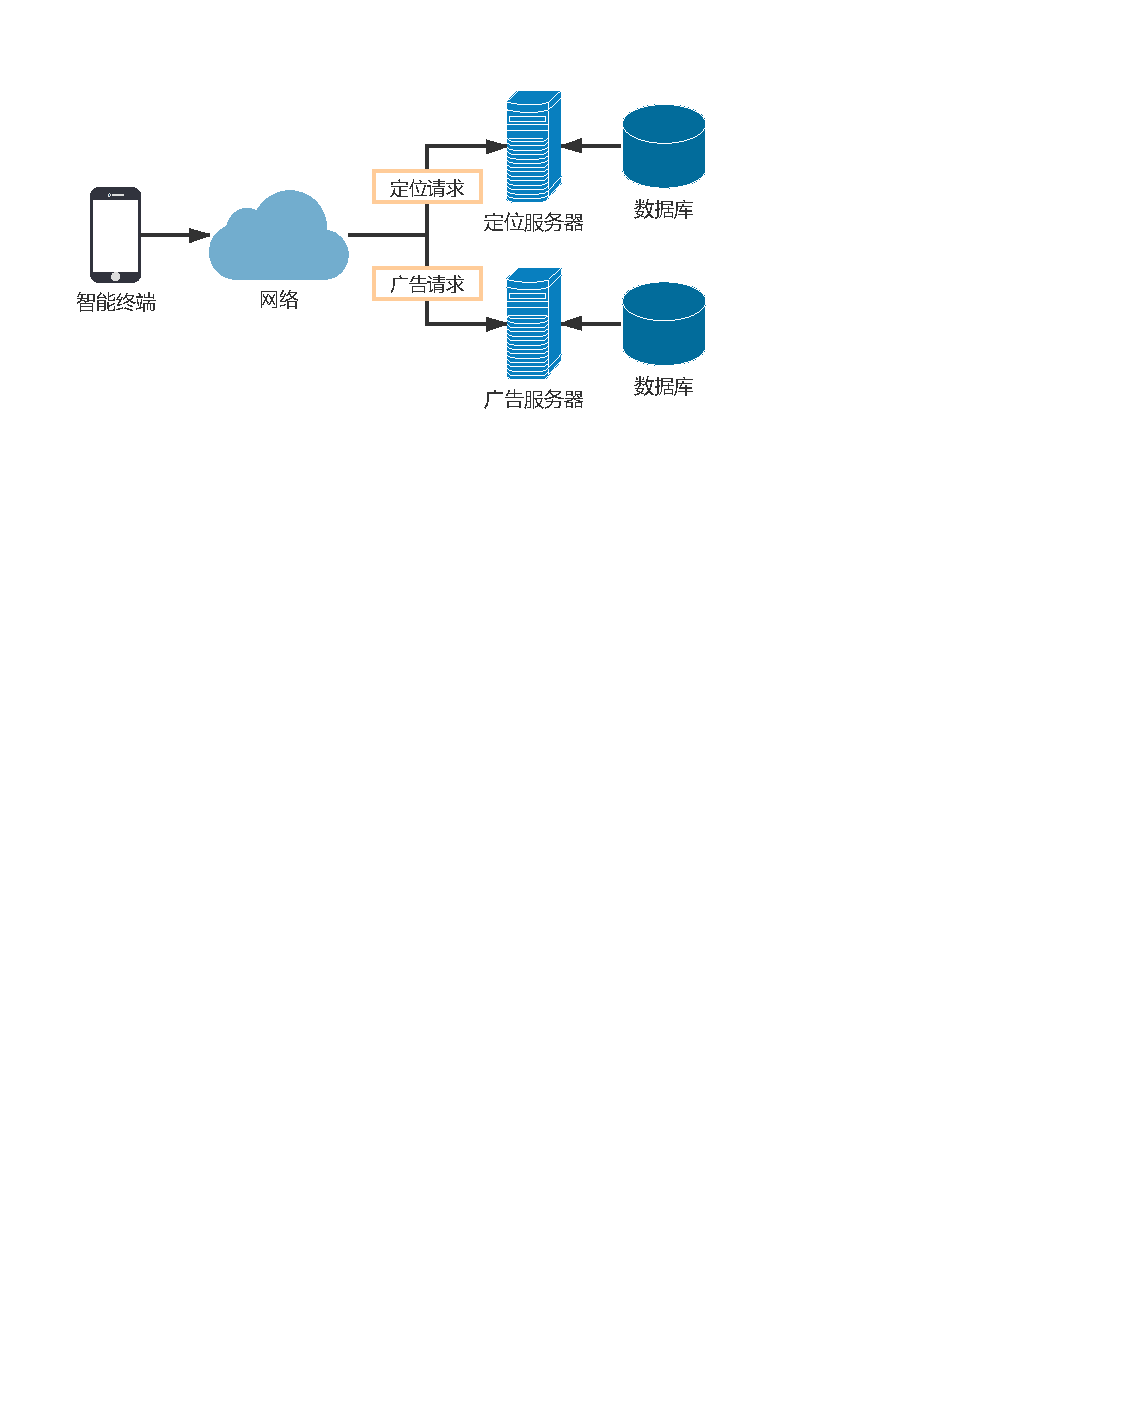
\includegraphics[width=\textwidth]{sys_arch.pdf}
	\caption{基于用户定位的广告投放服务机制的整体系统架构图。}
	\label{fig:sysarch}
\end{figure}

图\ref{fig:sysarch}所示为基于用户定位的广告投放系统总体框架。该系统由两大模块构成:定位服务模块和广告服务模块。每次用户访问该系统时,智能终端会先向定位服务器发送定位请求,定位服务器根据用户是信号发射源或接收端采取不同的算法计算用户位置,之后返回给终端。获得位置后,终端将向广告服务器发送广告请求,服务器计算完成后返回要投放给用户的广告。该系统主要由以下两个模块组成:
\begin{itemize}
	\item 在定位模块中,定位服务器其实是定位服务器群,因为这一部分由多个子模块组成,第\ref{sec:loc}节将详细介绍其系统架构和模块功能。如果终端是信号发射源,则数据库中存储着WAP接收到的该终端的RSS;若终端是信号接收端,则数据库中存储着历史上不同位置的RSS。从数据库中提取的数据被发送到定位服务器计算定位,最后位置被返回给终端。
	\item 在广告模块中,和定位模块类似,也是广告服务器群,第\ref{sec:ad}节将详细介绍其系统架构和模块功能。数据库存储着广告的具体内容,即视频、图片或文本形式的广告内容,在广告服务器决定要投放的广告之后到数据库提取相应的广告内容,并推送给用户。
\end{itemize}

当然图\ref{fig:sysarch}所展示的结构只是多种可能实现中的一种,比如定位信息的获取不是必须从定位服务器获取,也可以是在终端本地计算获得(比如卫星定位),只不过本文所提出的两种定位算法均需要在服务器计算获得定位信息。

\section{定位服务器系统架构} \label{sec:loc}

\begin{figure}[htb]
	\centering
	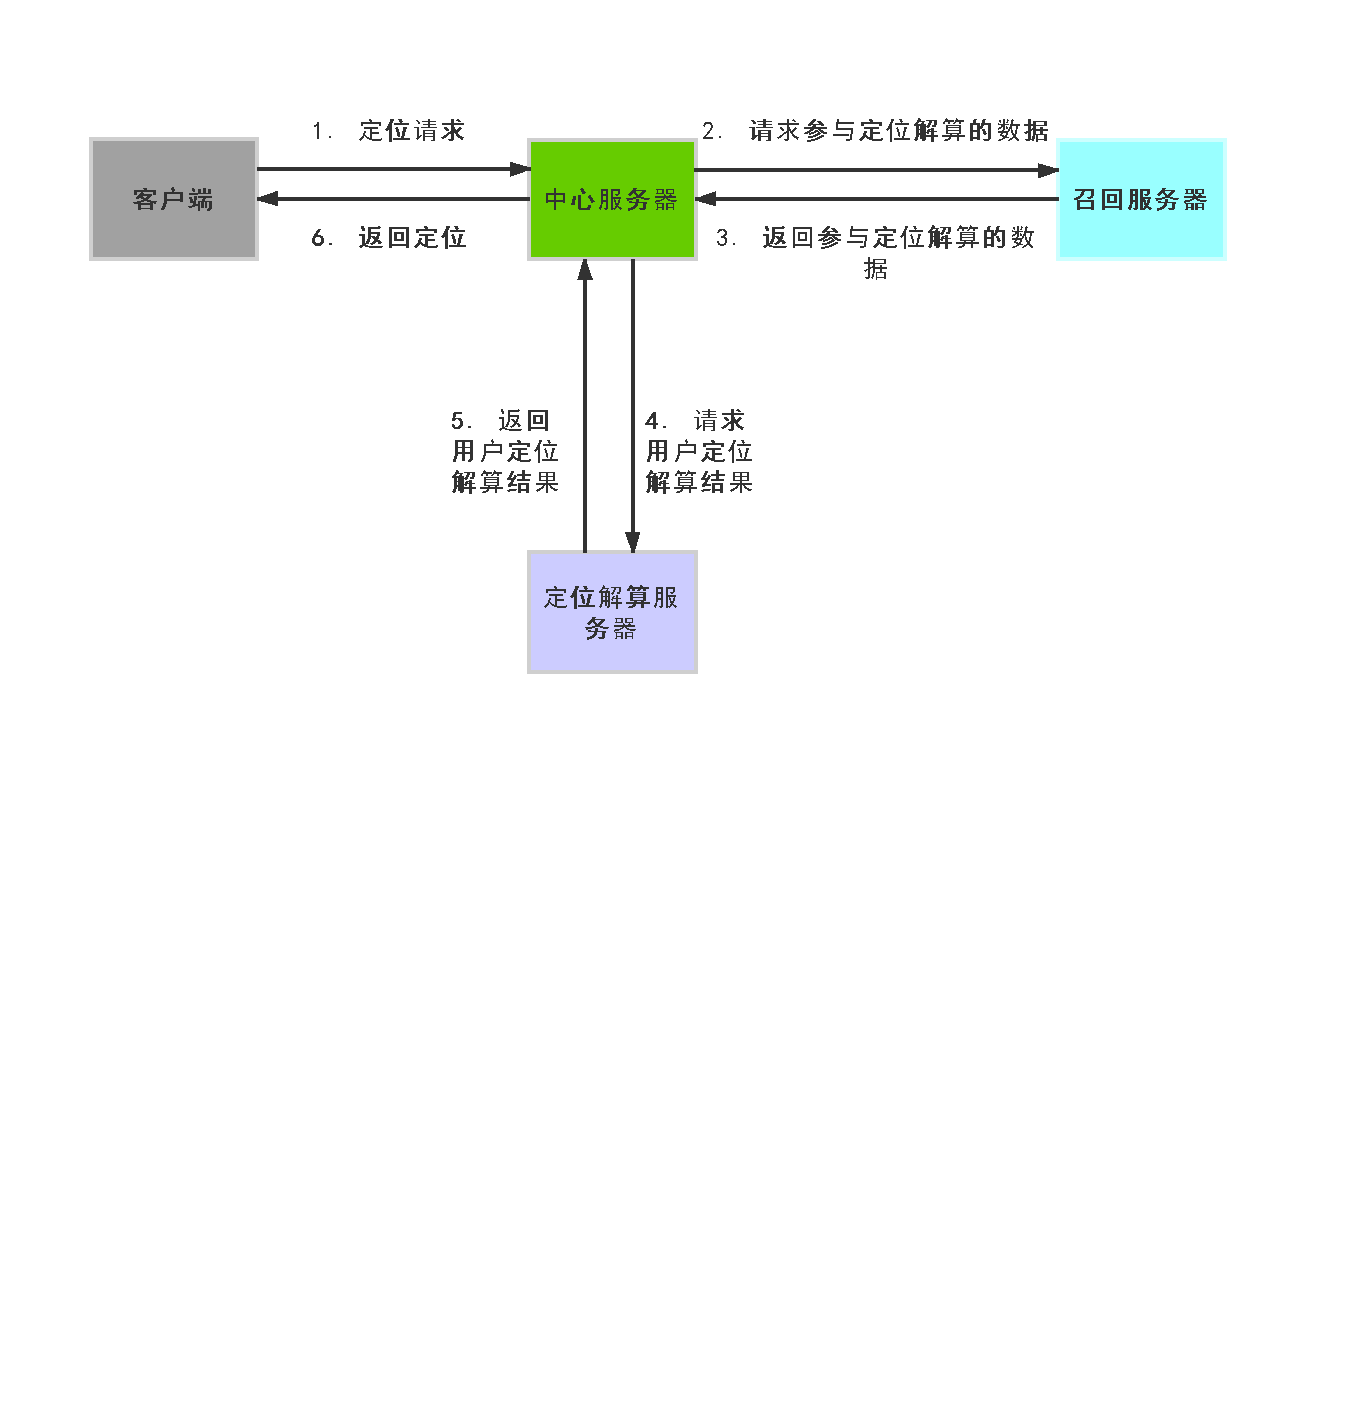
\includegraphics[width=\textwidth]{localization_process_cn.pdf}
	\caption{针对一次用户定位请求的工作流程图。}
	\label{fig:loc_sys}
\end{figure}

定位服务器(群)的具体结构如图\ref{fig:loc_sys}所示。每次客户端发起定位请求,中心服务器将依次从召回服务器取得数据、从定位解算服务器获取用户的定位信息,最后将用户位置返回终端。这里,中心服务器、召回服务器和定位解算服务器共同构成了定位服务器群。定位服务器依次执行的三步操作如下:
\begin{enumerate}
	\item 数据召回。由于数据库中数据量巨大,然而真正和当前用户定位相关的数据并没有那么多,因此我们需要设计一种快速算法将这些相关数据筛选出来。针对发射源定位和接收端定位的两种场景,我们将采用不同的召回策略:
	\begin{itemize}
		\item 发射源定位召回策略。由于发射源定位需要的用户周围基站处对于用户发射信号的RSS,而且数据库的写入会存在较大的延迟(相比于定位可以容忍的延迟),因此这里我们的策略是,当收到用户的定位请求后,令能接收到该用户信号的WAP将其RSS发送到中心服务器,则实现了数据的召回;
		
		\item 接收端定位召回策略。我们的接收端定位算法采用的是指纹定位,即利用附近WAP对用户的RSS与其所在区域的历史RSS数据进行匹配,用某种算法估计当前用户的位置。由于用户需要向定位服务器发送其RSS,因此我们知道用户能接收到哪些WAP的信号,据此可以在数据库中筛选出同时能够接收到这些WAP信号的点,或者适当放宽条件,可以接收到其中$1-\epsilon (0 < \epsilon < 1)$个WAP的点就被召回。这些数据将用作后续的匹配算法中;
	\end{itemize}
	
	\item 定位解算。这一部分是第\ref{cha:transmitter}章和第\ref{cha:fingerprint}章主要描述的内容,分别对应发射源定位和接收端定位。中心服务器将被召回的数据(如果是接收端定位,则还有用户的RSS数据)发送给定位解算服务器,根据定位的类型采取不同的算法解算用户位置。计算完成后,将用户位置返回给中心服务器;
	
	\item 最后,中心服务器通过网络将用户位置返回客户端。
\end{enumerate}

上述定位服务器架构只是一种可能的实现方式,比如当定位范围很小、数据较少的时候则可以省去数据召回的步骤,直接进行定位解算。这些其他的可能的架构在这里就不再赘述。

\section{广告服务器系统架构} \label{sec:ad}

\begin{figure}[htb]
	\centering
	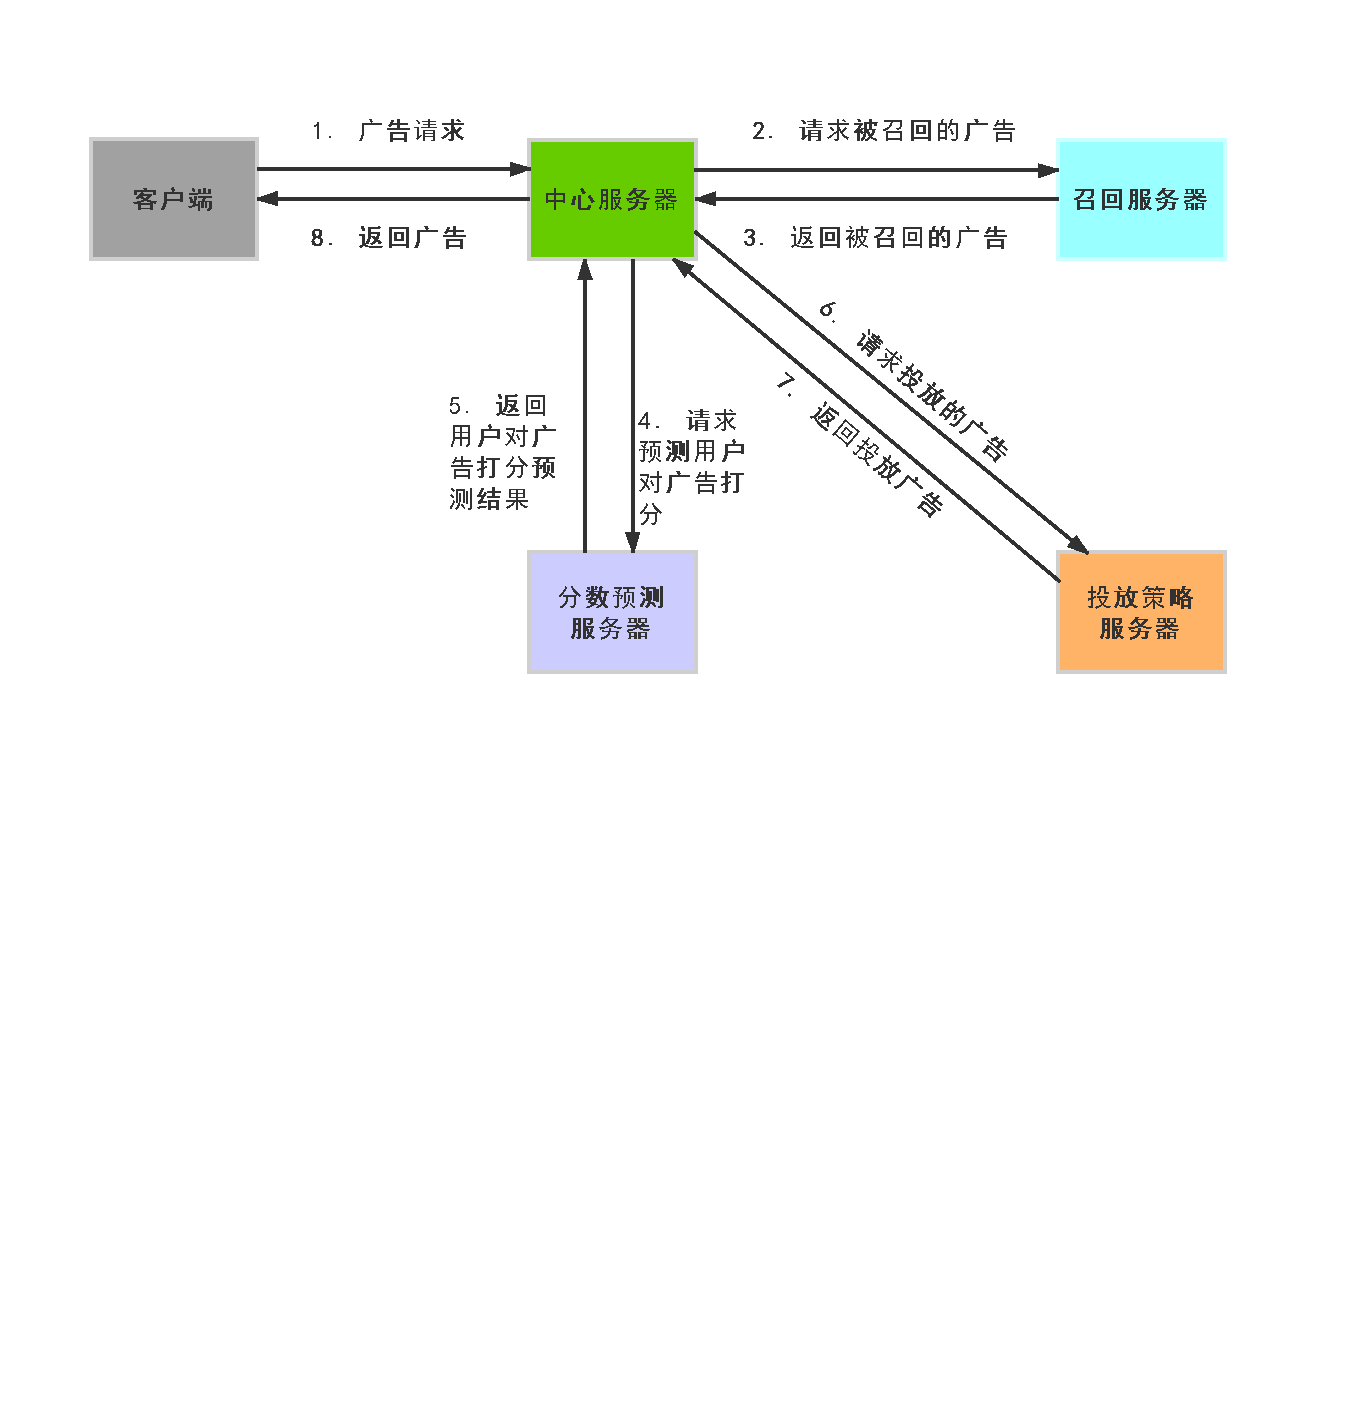
\includegraphics[width=\textwidth]{FansTop_process_cn.pdf}
	\caption{针对一次访问投放广告的工作流程图。}
	\label{fig:fssys}
\end{figure}

广告服务器(群)的具体结构如图\ref{fig:fssys}所示。流程从客户端发起广告请求开始,之后中心服务器依次请求召回广告、预测用户对被召回广告的打分和打算投放的广告。我们的算法将部署在投放策略服务器上。中心服务器、召回服务器、分数预测服务器和投放策略服务器共同构成了广告服务器群。广告服务器依次执行的四步操作如下:
\begin{enumerate}
	\item 广告召回。因为广告数量与服务器计算能力之间的矛盾,只有部分广告会参与后续流程,这个粗略过滤的操作被称作“召回”(Retrieval)或“候选集生成”(Candidate Generation)。不同于定位服务器中的召回服务,这里召回的是候选投放的广告,而定位中召回的相关、可以参与定位的历史数据。因为我们的算法要部署在同城页,这里仅介绍同城页的广告召回策略,即候选广告是根据访问用户与广告主之间的距离筛选的,也就是需要用到上文的定位信息。为了保证广告主得到他期望的曝光量,首先我们就得保证该条广告的召回量充足。为此,我们设置了几个距离等级,如果召回量太少就扩大召回范围,反之则缩小范围,使得广告召回量处在动态平衡中,既不会无法完成广告投放,又可以是得被投放广告的用户尽量靠近广告主;
	\item 分数预测。在被召回广告返回后,中心服务器会向分数预测服务器发送请求,以预测这些用户对于这些被召回广告的打分。预测服务器会根据广告特征、用户特征,以及用户过往行为等数据对当前广告预测分数。更详细的,预测服务器会返回CTR和条件关注率(Conditional Follow Rate, CFR)的线性组合:
	\begin{equation}
		score = CTR \times  (b + a \times CFR), \label{eq:score}
	\end{equation}
	其中 $a$ 和 $b$ 是线性组合系数,这里的条件关注率CFR是指在用户已经点击广告的条件下,用户关注广告主的概率,即分数可以被改写为:
	\begin{equation}
	score = b \times CTR + a \times FTR), 
	\end{equation}
	预测服务器会分别预测出\eqref{eq:score}中的CTR和CFR,之后返回分数。预测CFR而不是直接预测FTR的原因可能是一般FTR都比较小,直接预测的准确率较低;
	\item 投放广告,这也是第\ref{cha:allocation}章主要描述的部分。中心服务器在向投放策略服务器请求要投放的广告的同时,也会把召回的广告及其分数一起发送。计算完成后返回给中心服务器决定投放的广告。我们的算法和之前部署的流控算法唯一区别就在投放策略服务器上;
	\item 获取广告内容后,中心服务器将广告返回客户端。
\end{enumerate}

上述流程和框图是广告服务器的大致框架。限于篇幅原因,其他一些与算法无关的底层实现将不会在这里讨论。





